%
% File naaclhlt2010.tex
%
% Contact: nasmith@cs.cmu.edu

\documentclass[11pt,letterpaper]{article}
\usepackage{naaclhlt2010}
\usepackage{times}
\usepackage{latexsym}
\usepackage{graphicx}
\usepackage{url}
\setlength\titlebox{6.5cm}    % Expanding the titlebox

\newlength{\rhwidth}
\newcommand{\planaction}[3]{
\begin{minipage}{.5\textwidth}
\footnotesize
\setlength{\rhwidth}{.5\textwidth}
\addtolength{\rhwidth}{2.0cm}
{#1:}

\noindent \hspace{.2cm} \begin{minipage}{1.5cm}{Precond:}\end{minipage}\begin{minipage}[t]{\rhwidth} #2 \end{minipage}

\noindent \hspace{.2cm} \begin{minipage}{1.5cm}{Effect:}\end{minipage} \begin{minipage}[t]{\rhwidth}\ #3 \end{minipage}
\end{minipage}
}

\newcommand{\cplanaction}[4]{
\begin{minipage}{.5\textwidth}
\footnotesize
\setlength{\rhwidth}{.5\textwidth}
\addtolength{\rhwidth}{2.0cm}
{#1:}

\noindent \hspace{.2cm} \begin{minipage}{1.5cm}{Precond:}\end{minipage}\begin{minipage}[t]{\rhwidth} #2 \end{minipage}

\noindent \hspace{.2cm} \begin{minipage}{1.5cm}{Effect:}\end{minipage} \begin{minipage}[t]{\rhwidth} #3 \end{minipage}

\noindent \hspace{.2cm} \begin{minipage}{1.5cm}{Cost:}\end{minipage} \begin{minipage}[t]{\rhwidth} \ensuremath{#4} \end{minipage}
\end{minipage}
}



\title{Sentence Generation as Planning with Probabilistic LTAG\\
%\Thanks{}
}

\author{Daniel Bauer\\
  Columbia University\\
  New York, NY, USA\\
  {\tt bauer@cs.columbia.edu} 
  \And
  Alexander Koller\\
  Saarland University\\
  Saarbr\"{u}cken, Germany\\ 
  {\tt koller@mmci.uni-saarland.de}}

\date{}

\begin{document}
\maketitle

\input abstract

\section{Introduction} \label{sec:intro}

% What we'll do here.  Problem: RMRS is designed to support building
% semantic components to shallow parsers, and is intended to offer a way
% of integrating semantic representations
% computed by deep and shallow parsing.  We demonstrate the feasibility
% of this for the first time, by introducing a model theory for RMRS,
% defining entailment among RMRS representations and characterising this
% entailment relation 
% syntactically as extension of solved forms (ref to solved forms).  
% We show that the ``compatability'' of
% deep and shallow semantic representations is definable in terms of the
% entailment 
% relation between the RMRS
% representations.

% just so we have a citation here: \cite{Copestake_etal:MRS}

Representing semantics as a logical form that supports automated
inference and model construction is vital for deeper language
engineering tasks, such as dialogue systems.
These need access to the vast array of
semantic information that is captured in conventional logical forms,
including (but not limited to) information about semantic scope and
predicate argument structure.  Hand-crafted grammars yield detailed
logical forms (e.g., \cite{butt:etal:1999,copestake:flickinger:2000}), but deep parsing tends to lack
robustness: hand-crafted grammars fail to cover all words and
linguistic constructions; and unedited text and speech contains
ill-formed phrases, which by design deep grammars do not handle.  
\hidden{
Deep
parsers on their own also lack ambiguity resolution techniques,
producing all possible analyses.  Integration of statistical parse
selection with deep parsing is promising (e.g.,
\cite{toutanova:etal:2004}), but is not a solved problem.
}

Robost language processors that produce a single conventional logical
form for a given natural language string are beginning to emerge
(e.g.,
\cite{bos:etal:2004,rupp:etal:2000,wong:mooney:2006,zettlemoyer:collins:2005}).
But the output of these systems don't relate to any gold standard deep
parse as produced by expert grammar developers (for instance, while
the training corpus used in \cite{zettlemoyer:collins:2005} features
control phenomena in the language strings, their logical forms don't
represent it).  This makes it hard to judge the logical forms that the
models derive from a linguistic perspective; nor can one integrate
their output with that of a hand-crafted grammar when desired.

This paper focusses on a particular approach to producing semantic
information from robust parsers, exemplified in
\cite{copestake:2003,frank:2004}, among others.  Their strategy is to
utilise semantic underspecification to semi-automatically build
semantic components to shallow parsers, so that the output neither
over-determines nor under-determines the semantic information that is
revealed by the (shallow) syntactic analysis.  The semantic formalism
used to express this is Robust Minimal Recursion Semantics ({\sc
  rmrs}, \cite{copestake:2003}); this is an extension of {\sc mrs}
\cite{copestake:etal:2005} that is designed to be maximally flexible
in the type of semantic information that can be left underspecified:
it can express partial information about semantic scope, the values of
arguments to predicate symbols and/or their argument position, the
arity of the predicate symbols and the sorts of arguments they take.
We show in Section~\ref{sec:motivation} that all these features are
needed when information about lexical subcategorisation or
syntactic dependencies is missing---a characteristic feature of
shallow parsers.  Several researchers have demonstrated that {\sc
  rmrs} is a suitable framework on which to semi-automatically
construct semantic components to shallow parsers, ranging in depth
from {\sc pos} taggers (refs) to chunk parsers (frank ref) and
intermediate parsers ({\sc rasp} ref).

A major motivation for adopting {\sc rmrs} over other techniques for
robustly deriving logical forms is the promise that it can form the
basis for integrating the output of several parsers, and be compared
in particular with the output of a hand-crafted grammar.  This paper
demonstrates the feasibility of this integration for the first time,
by introducing a model theory for {\sc rmrs}, that in turn defines
entailment among {\sc rmrs} representations.  This entailment relation
is also characterised syntactically as an extension of solved forms
(ref to solved forms).  We show that the proof theory and model theory
of {\sc rmrs} that results provides a formal basis for integrating the
semantic output of several shallow parsers, for checking the
satisfiability of a shallow parse, and for testing its compatibility
with a deep parse.

%%% Local Variables: 
%%% mode: latex
%%% TeX-master: "rmrs-08"
%%% End: 

\section{A unified perspective on GRE} \label{sec:related}

\begin{figure}
  \centering
  \begin{tabular}{l|l}
    GRE algorithm & DL variant \\ \hline
    \newcite{Dale1995} & $\mathcal{CL}$ \\
    \newcite{deemter01:_gener_refer_expres} & $\mathcal{PL}$ \\
    \newcite{dale91:_gener_refer_expres_invol_relat} & \el \\
    \newcite{Krahmer2003} & \el \\
    \newcite{kelleher06:_increm_gener_of_spatial_refer} & \el \\
    \newcite{gardent02:_gener_minim_defin_descr} & $\mathcal{ELU}_{(\neg)}$
  \end{tabular}
  \caption{DL variants used by different GRE algorithms.}
  \label{fig:related}
\end{figure}

Viewing GRE as a problem of generating DL concepts offers a new,
unified perspective of the GRE problem: It is the problem of computing
a DL concept with a certain (typically singleton) extension.  Many
existing approaches can be subsumed under this view; we have
summarized this for some of them in Fig.~\ref{fig:related}, along with
the DL fragment they use.  We already discussed some of these
approaches in Section~\ref{sec:gre}.  Furthermore, the graphs
\newcite{Krahmer2003} use to represent referring expressions can be
seen as concepts of \el\ that are only satisfied at those points at
which they can be embedded; the non-relational but negative and
disjunctive descriptions generated by
\newcite{deemter01:_gener_refer_expres} are simply concepts of
$\mathcal{PL}$; and \newcite{gardent02:_gener_minim_defin_descr} then
generalizes this into generating concepts of $\mathcal{ELU}_{(\neg)}$,
i.e.\ \el\ plus disjunction and atomic negation.

The approach presented here fits very well into this landscape, and in
a sense completes the picture by showing how to generate concepts for
arbitrary bisimulation classes in \alc, which combines all connectives
used in any of these previous approaches.  Where our approach breaks
new ground is in the way these concepts are computed: It successively
refines a decomposition of the domain into subsets.  In this way, it
is reminiscent of the Incremental Algorithm, and in fact the IA can be
seen as the special case of the \el\ algorithm for the non-relational
case.

However, our approach is in contrast with
\newcite{dale91:_gener_refer_expres_invol_relat} and its successors,
such as \newcite{kelleher06:_increm_gener_of_spatial_refer}, which
attempt to generate a RE for a single individual for successive
individuals in the model and therefore run a risk of infinite regress.
Our algorithms are guaranteed to terminate (and with concepts of the
smallest relational depth that cover all the data), and infinite
regress is automatically excluded.  Perhaps closest in spirit is the
Krahmer et al.\ graph algorithm, which also computes \el\ concepts by
extending them successively; but this algorithm, too, is focused on
reference to a single individual, and it has NP-complete worst-case
complexity.







%%% Local Variables: 
%%% mode: latex
%%% TeX-master: "dl-gre-08"
%%% End: 
 % Related work
\section{Sentence generation as planning}
\label{sec:crisp}


We consider a planning domain that comes up in the generation of
natural language sentences based on tree-adjoining grammar (TAG;
\cite{joshi;etal1997}).  This is a standard problem in computational
linguistics, which we sketch by example; see
\cite{Stone2003a,KolSto07} for details.

% \begin{figure}
%   \centering
%   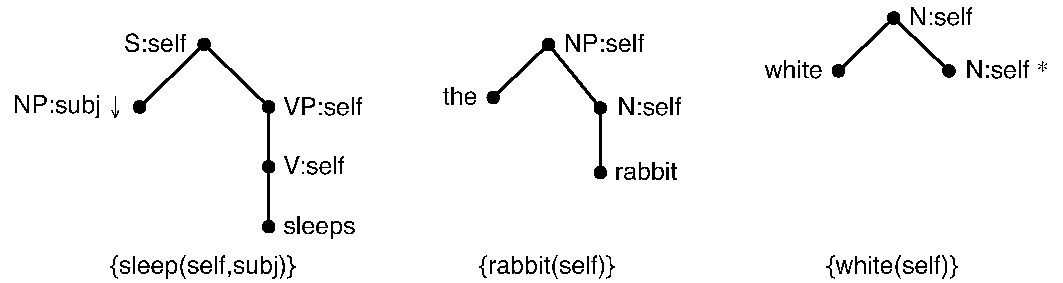
\includegraphics[width=0.75\columnwidth]{pic-grammar}
%   \caption{An example grammar in the sentence generation domain.}
%   \label{fig:white-rabbit-sleeps-grammar}
% \end{figure}

\begin{figure}
  \centering
  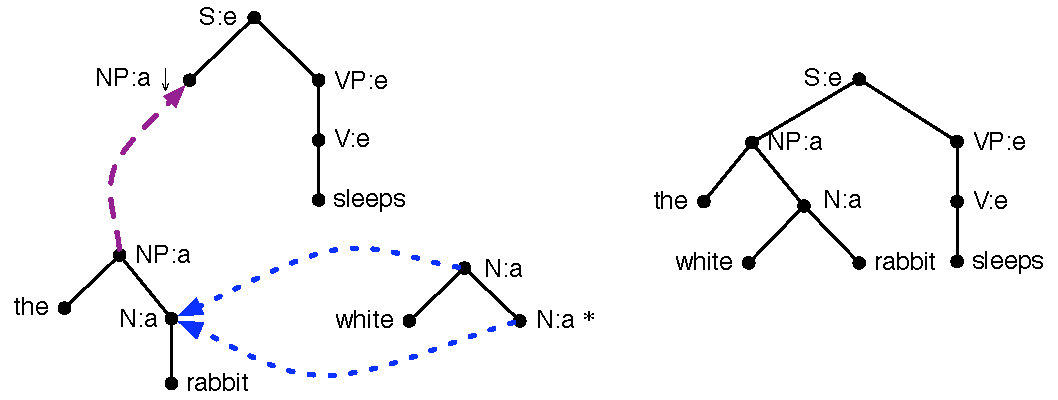
\includegraphics[width=1\columnwidth]{pic-derivation}
  \caption{Derivation of ``The white rabbit sleeps.''}
  \label{fig:white-rabbit-sleeps-deriv}
\end{figure}

A TAG grammar consists of a finite set of \emph{elementary trees},
each of which contains one or more words; the left of
Fig.~\ref{fig:white-rabbit-sleeps-deriv} shows three trees for ``the
rabbit'', ``sleeps'', and ``white''.  Trees can be combined using the
operations of \emph{substitution} (purple dashed arrow in the figure)
and \emph{adjunction} (blue dotted arrows) to form larger trees.
The end result of a grammatically correct derivation is a tree all of
whose leaves are labeled with words, as on the right of
Fig.~\ref{fig:white-rabbit-sleeps-deriv}. We can read off a sentence
from such a tree from left to right.

To use TAG grammars for generation \cite{Stone2003a}, we assume a set
of ground atoms expressing the information we want the sentence to
convey, such as $\{\mathsf{sleep}(e,r_1)\}$, and a knowledge base that
contains all ground atoms we know to be true; say,
$\{\mathsf{sleep}(e,r_1), \mathsf{rabbit}(r_1), \mathsf{rabbit}(r_2),
\mathsf{white}(r_1), \mathsf{brown}(r_2)\}$.  We then add variables
ranging over constants from the knowledge base to the nodes of each
elementary tree, and equip every elementary tree with a set of atoms
over these variables to encode the meaning this tree expresses.
Fig.~\ref{fig:white-rabbit-sleeps-deriv} already shows specific
instances of the elementary trees from the grammar, in which constants
have been substituted for these variables.  The derivation in the
figure conveys the intended meaning -- in particular, that $r_1$
sleeps.  Crucially, it also describes uniquely who does the sleeping:
The sentence ``the rabbit sleeps'' would not have done this, as ``the
rabbit'' could be understood either as $r_1$ or $r_2$.  We say that
$r_2$ is a \emph{distractor} for the subject of the sentence, which is
removed by adjoining the tree for ``white''.  The sentence generation
problem consists in computing a grammatically correct TAG derivation
from instances of the elementary trees in the grammar that conveys the
intended meaning and describes all referents uniquely.




\subsection{Sentence generation as a planning problem}

The TAG sentence generation problem can be encoded as a planning
problem \cite{KolSto07}.  The key idea is that each operator encodes
the addition of an elementary tree to the derivation; the syntactic
and semantic requirements and effects of doing this are captured in
the operator's precondition and effect.


\newcommand{\action}[4]{\textbf{#1$(#2)$:}\\
\strut\quad   Precond:$\;$ \parbox[t]{12cm}{\ensuremath{#3}}\\
\strut\quad   Effect:$\;$ \parbox[t]{12cm}{\ensuremath{#4}}}
\newcommand{\f}[1]{\mathsf{#1}}

\begin{figure}
%\centering
%\begin{minipage}{0.8\textwidth}
{\small%
\action{sleeps}{u, u_1, u_n, x_0, x_1}{
  \f{subst}(\f{S},u) \wedge \f{ref}(u,x_0) \wedge
  \f{sleep}(x_0,x_1) \\ \wedge \f{current}(u_1) \wedge
  \f{next}(u_1,u_n)
}{
  \neg \f{subst}(\f{S},u) \wedge \f{expressed}(\f{sleep}, x_0, x_1) \\
  \wedge \f{subst}(\f{NP},u) \wedge \f{ref}(u_1,x_1) \\ \wedge
  \neg \f{current}(u_1) \wedge \f{current}(u_n) \\ \wedge
  \forall y. y \neq x_1 \rightarrow \f{distractor}(u_1,y)
}\\

\action{rabbit}{u, x_0}{
  \f{subst}(\f{NP},u) \wedge \f{ref}(u,x_0) \wedge \f{rabbit}(x_0)
}{
  \neg \f{subst}(\f{NP},u) \wedge \f{canadjoin}(\f{N},u) \\
  \wedge \forall y. \neg \f{rabbit}(y) \rightarrow \neg \f{distractor}(u,y)
}\\

\action{white}{u,x_0}{
  \f{canadjoin}(\f{N},u) \wedge \f{ref}(u,x_0) \wedge \f{rabbit}(x_0)
}{
  \forall y. \neg \f{white}(y) \rightarrow \neg \f{distractor}(u,y)
}
}\strut\\[-5ex]
%\end{minipage}
\caption{Actions for generating ``The white rabbit
sleeps.''}
\label{fig:white-rabbit-as-planning}
\end{figure}

More precisely, each operator has a parameter $u$ representing the
syntax node into which the elementary tree is substituted or adjoined,
and a parameter $u_i$ for each substitution node.  There are also
parameters $x_0,\ldots,x_k$ for the variables in the semantic
representation of the elementary tree; $x_0$ is the variable that
occurs at the root of the tree.  The planning state encodes a list of
possible node names; $\f{current}(u)$ expresses that $u$ is the next
node name that should be picked when a new substitution node is
created, and $\f{next}(u,v)$ says that the next node after $u$ is
$v$. These atoms are used to select names for the substitution nodes
that are introduced by adding an elementary tree; the parameter $u_n$
represents the node that will be current after the addition.

The atom $\f{subst}(A,u)$ expresses that we need to still substitute
something into the substitution node $u$ with label $A$; the initial
state contains an atom $\f{subst}(\f{S},\f{root})$ where $\f{S}$
stands for ``sentence'' and $\f{root}$ is an arbitrary name for the
root of the derivation.  The mapping from nodes to semantic constants
is maintained using the $\f{ref}$ atoms; the initial state for
generating a sentence about the event $e$ contains an atom
$\f{ref}(\f{root},e)$.  Finally, we keep track of the uniqueness of
referring expressions in the $\f{distractor}$ atoms:
$\f{distractor}(u,a)$ expresses that the expression at syntax node $u$
could still be misunderstood as $a$.

The example generation problem above translates into a planning
problem whose domain is shown, in PDDL format, in
Fig.~\ref{fig:white-rabbit-as-planning}. The initial state of the
problem encodes the generation problem's knowledge base; it contains
atoms $\f{rabbit}(r_1)$, $\f{sleep}(e,r_1)$, etc.  The goal requires
syntactic completeness as $\forall u \forall A \neg \f{subst}(A,u)$
and unique reference as $\forall u \forall x \neg
\f{distractor}(u,x)$; it also specifies the semantic representation we
want to express in an atom $\f{expressed}(\mathsf{sleep},e,r_1)$.

A minimal plan for the example problem is
$\mathsf{sleeps}(\mathsf{root}, n_1, n_2, e, r_1)$;
$\mathsf{rabbit}(n_1, r_1)$; $\mathsf{white}(n_1, r_1)$. This plan can
be automatically decoded into the derivation shown in
Fig.~\ref{fig:white-rabbit-sleeps-deriv}.  The analogous plan with
$r_2$ instead of $r_1$ is not correct because the $\mathsf{sleep}$
precondition of the $\mathsf{sleeps}$ operator is not satisfied.  The
first two steps of the plan alone would not be a correct plan because
they leave an atom $\mathsf{distractor}(n_1, r_2)$ in the state, which
contradicts the goal that all distractors have been eliminated.






%%% Local Variables: 
%%% mode: latex
%%% TeX-master: "main"
%%% End: 
 % Sentence Generation as Planning
\section{Statistical Generation as Planning}
\label{sec:pcrisp}

We now extend \crisp\ to statistical generation (\pcrisp). The basic idea is to add a statistical grammar model while leaving the sentence generation mechanism untouched. This way we can select the highest scoring derivation which satisfies all constraints (grammaticality, expresses the communicative goal, uses unambiguous referring expressions, etc.). 

 As a straightforward probability model over {\sc ltag} derivations we choose probabilistic {\sc tag} ({\sc ptag}) \cite{resnik1992}.
Our choice of {\sc ptag} for sentence generation is motivated by a number of attractive properties.
 {\sc Ptag} is lexicalized and therefore does not only assign probabilities to operations in the grammar (as for example plain {\sc pcfg}), but also accounts for binary dependencies between words.  Unlike n-gram models however, these co-occurrences are structured according to local syntactic context as a result of {\sc tag}'s extended domain of locality. The probability model describes how the syntactic arguments of a word are typically filled. 
Furthermore, as {\sc tag} factors recursion from the domain of dependencies, the probability for core constructions remains the same independent of additional adjunctions. 
%Second, {\sc ptag} is a generative model. This is crucial because it allows us to assign probabilities to partial derivations. In addition we use the probability of partial derivations as a cost function, to help guide search through the space of possible PLTAG derivations. In contrast, other statistical generation systems use discriminative models that select the best possible generation output from a set of candidate sentences.
%Finally, the independence assumption makes it easy to estimate {\sc ptag}s from a treebank.
 We review {\sc ptag} in section \ref{ssec:probmodels}.

While we leave the basic sentence generation mechanism intact, we need to modify the concrete formulation of \crisp\ planning operators to accommodate bilexical dependencies. Likewise, we need to take the step from classical planning to \emph{metric} planning systems which can use the probabilities.
In metric planning \cite{fox2002}, planning actions can modify the value of numeric variables in addition to adding and deleting logical literals to the state. The goal state specifies constraints on this variable. In the simplest case the variable can only be increased by a static cost value in each action, and the goal state contains the objective to minimize the total cost. While systems such as Metric-{\sc FF} \cite{hoffmann2003} do not guarantee optimality, they do generally offer good results. We address our encoding of sentence generation with {\sc ptag} as metric planning in section \ref{ssec:pcrisp-domains}. 

\subsection{Probabilistic TAG}
\label{ssec:probmodels}
{\sc ptag} \cite{resnik1992} views {\sc tag} derivations as sequences of events of three types: initial events, substitution events, and adjunction events.

The probability distribution for initial events describes how likely it is to start any derivation with a given initial tree. 
It is defined over all initial trees $\alpha \in I$ with their possible lexicalizations $w \in W_\alpha$: 
$$ \sum\limits_{\alpha \in I}\sum\limits_{w \in W_\alpha} P_i(\init(\alpha, w)) = 1 $$

For substitution events, there is a probability distribution for each substitution node $n$ of each elementary tree $\tau$ lexicalized with $v$, which describes how likely it is to substitute it with an initial tree $\alpha$ lexicalized with $w$. 
$$\sum\limits_{\alpha \in I}\sum\limits_{w \in W_\alpha} P_s(\subst(\tau,v , \alpha, w, n)) = 1$$

Similarly for each internal node there is a distribution that describes the probability to adjoin an auxiliary tree $\beta \in A$ lexicalized with $w$. In addition some probability mass is reserved for the event of not adjoining anything to such a node at all.

$$ P_a(\noadj(\tau, v, n)) + \strut$$
$$ \sum\limits_{\beta \in A}\sum\limits_{w \in W_\beta} P_a(\adj(\tau, v, \beta, w, n)) = 1.$$

{\sc Ptag} assumes that all events occur independently of each other. Therefore it defines the total probability for a derivation as the product of the probability of its individual events. 

\subsection{PCRISP Planning Domains}
\label{ssec:pcrisp-domains}
Using the definition of {\sc ptag}, we now reformulate the \crisp\ planning operators described in section \ref{ssec:crispdomain}.
The independence assumption in {\sc ptag} allows us to continue to model each addition of a single elementary tree to the derivation (with a certain probability score). However, while \crisp\ planning operators can add an elementary tree to any site of the correct category, {\sc ptag} substitution and adjunction events are binary events between lexicalized trees at a specific node. We therefore adapt the literals that record open substitution and adjunction sites in partial derivations accordingly and create one operator for each node in each possible combination of lexicalized trees.
Fig.~\ref{example-action} shows an example planning operator for each type.
\begin{figure}[t]
\begin{center}
\cplanaction{\bf subst-t3-cat-t28-eats-n1(u,~x1)}{referent(u,~x1),\\ subst(t28-eats,~n1,~u), cat(x1)}{
$\lnot$needtoexpr(pred-cat,~x1),\\ $\lnot$subst(t-28-eats, n1,~u),\\
adj(t3-cat, n2 u)}{4.3012}\\\smallskip

\cplanaction{\bf adj-t5-raw-t3-fish-n2(u,~x1)}{referent(u,~x1),\\ adj(t28-eats,n2,~u), raw(x1)}{
$\lnot$needtoexpr(pred-raw,~x1),\\ $\lnot$adj(t-28-eats, n2,~u)}{6.9076}\\\smallskip

\cplanaction{\bf init-t28-eats(u,~x1,~x2,~x3)}{referent(u,~x1),\\ eats(x1,~x2,~x3)}{
$\lnot$needtoexpr(pred-eats,~x1,~x2,~x3), \\
 subst(t-28-eats,~n1,subj), subst(t28-eats,~n4,obj),\\
adj(t-28-eats, n2, u), adj(t-28-eats, n3, u)}{8.5172}\\\smallskip

\cplanaction{\bf noadj-t28-eats-n3(u)}{
 adj(t-28-eats,~n3,u)}
{$\lnot$ adj(t-28-eats, n3, u)}{0.1054}\\\smallskip

\caption{\label{example-action} Some \pcrisp\ operators for the grammar from Fig.~\ref{fig:grammar}.}
\end{center}
\end{figure}

Finally, we set the cost of an operator to be its negative log probability. For example 
\begin{align*}
&Cost(\mbox{subst-t3-cat-t28-eats-n1}) = \\
 & \qquad -\log P_s(\subst(\mathrm{t3},\textit{`cat'},\mathrm{t28},\textit{`eats'},\mathrm{n1})) ).
\end{align*}
This way the plan which minimizes the sum of the costs of its actions  corresponds to the {\sc tag} derivation with the highest probability. 

\subsection{Dealing with Data Sparseness}
\label{ssec:sparseness}
The event definition of {\sc ptag} is very-fine grained. Substitution and adjunction events depend on specific parent and child trees with specific lexicalizations and on a node in the parent tree, as illustrated in Fig.~\ref{fig:modelillustration}, B.1. When we estimate a probability model from training data, we cannot expect to observe evidence for all combinations of trees. Derivations that include such unseen events have zero probability and are therefore impossible. As we show in section \ref{sec:experiments}, this gives rise to a massive data sparseness problem.

  A straightforward way to deal with data sparseness is to drop all lexicalizations from event definitions, as illustrated in Fig.~\ref{fig:modelillustration}, A. Unfortunately this model  no longer accounts for bilexical dependencies between words. Since our system has to add a lexicalized tree in each step, lexicalizations for this child tree should always be taken into account by the probability model, if available. Despite these drawbacks, we perform experiments with the unlexicalized model as a baseline. This allows us to investigate if purely syntactic information is sufficient to achieve high quality generation output.

An alternative model computes linear interpolation between three back-off levels. The first level is just standard {\sc ptag} (Fig.~\ref{fig:modelillustration}, B.1), for the second level the lexicalizations of the parent tree is dropped (Fig.~\ref{fig:modelillustration}, B.2), for the third level the model describes only the distribution of lexicalized child trees over each category (Fig.~\ref{fig:modelillustration}, B.3).  
Notice also that the third level is similar in spirit to a probabilistic version of original \crisp\ operators (compare Fig.~\ref{fig:modelillustration}, B.3 and Fig.~\ref{fig:crisp-operators}). 
\begin{figure}[t]
\begin{center}
\includegraphics[width=.5\textwidth]{figures/modelillustration}
\caption{\label{fig:modelillustration} Illustration of the unlexicalized probability model (A) and the three back-off levels of the linear interpolation model (B).}

\end{center}
\end{figure}


%It is obvious that the number of total planning operators grows quadratically with the number of possible input words in the grammar. In practice this causes a problem for most heuristic search planners, which will instantiate planning operators to all possible actions before attempting to solve the problem. Our generation system therefore only selects operators that are compatible with the input semantics before running the planner. 
%On the other hand,


%\newcommand{\init}[0]{\textit{ init}}
%\newcommand{\subst}[0]{\textit{ subst}}

%\begin{figure}[p]
%\caption{\label{modelillustration} The three back-off levels.}
%\begin{center}
%\includegraphics[width=.5\textwidth]{modelillustration}
%\end{center}
%\end{figure}





%%% Local Variables:  %%% mode: latex %%% TeX-master: "pcrisp-10" %%% End:  % Statistical Generation as Planning
\section{Experiments} \label{sec:experiments}

We now describe the results of three simple experiments designed to
evaluate the suitability of particular planners (FF, SGPLAN, and an ad-hoc
implementation of GraphPlan) in our two NLG domains. As a first impression,
our results indicate that planning is a promising tool for both domains. In
the GIVE domain, SGPLAN 5.2.2 computes a domain plan from the initial state
to the goal in 0.3 seconds, which is fast enough for moderately-sized
problems instances in the application.\footnote{All runtimes were
  measured on a Pentium 4 CPU running at 3 GHz. Java programs were allowed
  to ``warm up'', i.e.\ the planner was run five times and the first four
  measurements discarded to ensure that the JVM had just-in-time compiled
  all relevant bytecode.}
In the sentence generation domain, FF dramatically outperforms the best
previously known algorithm for the same problem (a reimplementation of
\cite{Stone2003a}), although the latter is a greedy search algorithm with a
heuristic that is hand-tailored to the domain.

We also observe that although FF manages the search for a plan very
efficiently, it spends comparatively large amounts of time computing
instantiations of predicates and actions, most of which are then never used
during the search. As a result, FF's ``grounding time'' dominates its
overall planning time, leading to some conflicting results. Our experiments
below seek to improve our understanding of this situation.


\subsection{Experiment 1: Sentence generation}
\label{sec:exper-1:-sent}

In the first experiment, we generate a series of sentence generation
problems which require the planner to compute a plan representing the
sentence ``Mary likes the Adj$_1$ \ldots Adj$_n$ rabbit.''  Each problem
instance assumes a certain number $m$ of rabbits that were distinguished by
$n \leq m$ different properties, such that all $n$ properties are required
to distinguish the target referent from all other rabbits.  The $n$
properties are realized as $n$ different adjectives, in any order.  This
setup allows us to control the plan length (a plan with $n$ properties will
have length $n+4$) and the universe size (the universe will contain $m+1$
individuals in addition to the differently-typed individuals used to encode
the grammar).

\begin{figure}
  \centering
  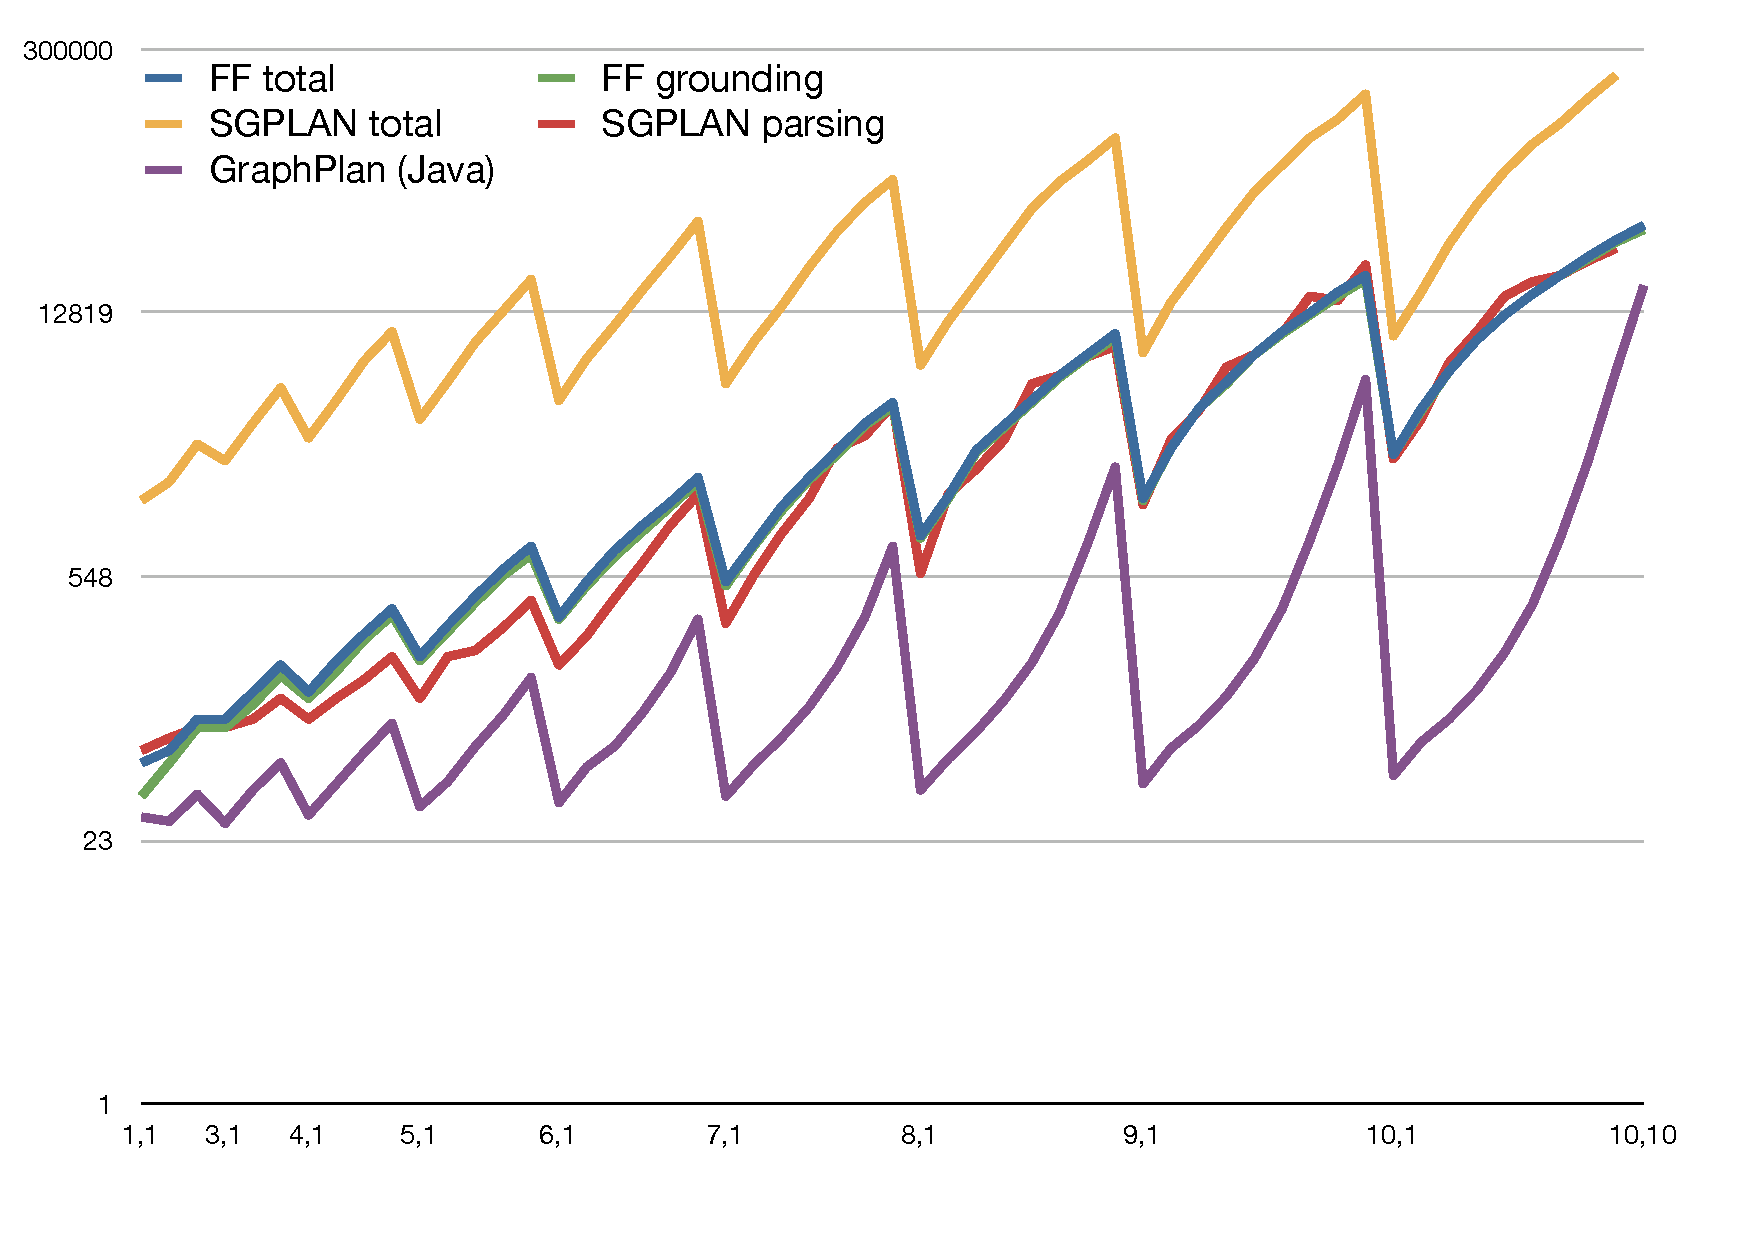
\includegraphics[width=1\columnwidth]{pic-runtime-modifiers-with-sgplan}
  \caption{Runtimes in the sentence generation domain. The horizontal
  axis represents parameters $(m,n)$ from $(1,1)$ to $(10,10)$ in
  lexicographical order.}
  \label{fig:runtimes-crisp}
\end{figure}

The results of this experiment are shown in
Figure~\ref{fig:runtimes-crisp}. The input parameters $(m,n)$ are plotted
(in lexicographic order) on the horizontal axis and the runtime is shown in
milliseconds on the vertical axis. These results reveal a number of
interesting insights. First, FF significantly outperforms
SGPLAN in this domain.\footnote{Experiments with SGPLAN use a
 pre-release version of SGPLAN, kindly provided by Chih-Wei Hsu. The
 release version of SGPLAN 5.2.2 had a bug, causing it to crash on some
 instances.}
Second, FF's runtime is dominated by its initial grounding step, in which
it computes the ground instances of all predicates and actions used in the
planning problem to avoid unnecessary instantiations during search. In
particular, the ratio of grounding time to total runtime is generally above
85\%, and rises to above 99\% at $m=11$, which is still a small universe in
this application.\footnote{The
  ``grounding'' time reported here is what FF reports as ``time spent:
  instantiating action templates''.}  This is also reflected in the
much higher sensitivity of FF to the domain size: if we fix $n=1$, FF takes
60 ms to compute a plan at $m=1$, but 2.4 seconds at $m=10$. By contrast,
our naive GraphPlan implementation takes 30 ms at $m=1$ and still only 50
ms at $m=10$.

Our results illustrate that FF is outperformed quite clearly by an ad-hoc
Java implementation of GraphPlan which only computes instances of
predicates and actions as they are discovered, while the planning graph is
being built. On the other hand, the runtime that FF actually spends on
search is again considerably lower than that of our GraphPlan
implementation, and for any given $m$, GraphPlan's runtime grows much
faster with $n$ (i.e., the plan size) than FF's. As a result, for
moderately-sized instances of the sentence planning domain FF does very
well on search, but spends about ten times as much runtime again on
grounding. Larger (but still realistically-sized) instances of the sentence
generation problem are still problematic for the planners we tested.



\subsection{Experiment 2: Minimal GIVE worlds}
\label{sec:exper-2:-minim}

In the second experiment, we evaluate the performance of the planners on
problems arising in the GIVE domain. We construct a series of test worlds,
similar to the one illustrated in Figure~\ref{fig:give-minimal}. These
worlds consist of a $2n$ by $h$ grid of positions, such that there are
buttons at positions $(2i-1,1)$ and $(2i,h)$ for $1 \leq i \leq n$. The
player starts in position $(1,1)$ and must press all buttons in order to
successfully complete the game. The world is generated as a GIVE world
description, and then automatically converted into a planning problem by
the GIVE software. (We refer the reader to \todo{add citation} for more
details about this process.)

\begin{figure}
  \centering
  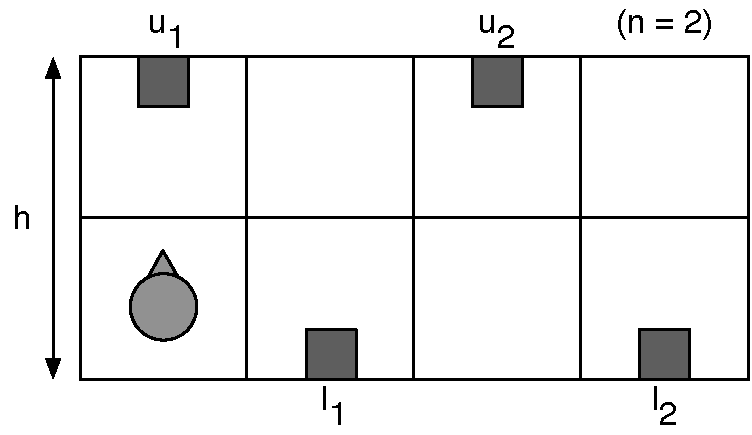
\includegraphics[width=0.8\columnwidth]{pic-buttons}
  \caption{Minimal GIVE world.}
  \label{fig:give-minimal}
\end{figure}

Results for the $h=20$ case, with $n$ ranging from $1$ to $40$, are shown
in Figure~\ref{fig:give-runtime-minimal}.  The most obvious result is that
FF is unable to solve any problems beyond $n=13$ on our experimentation
machine within the memory limit of 1 GB.  SGPLAN, on the other hand, solves
instances beyond $n=40$ without major problems.  The time spent on
grounding is not a major factor in either planner, probably because the
planners need more time to actually compute the plan---for instance, the
optimal plan for the problem $n=40$ has a length of about 1600 steps.

\begin{figure}
  \centering
  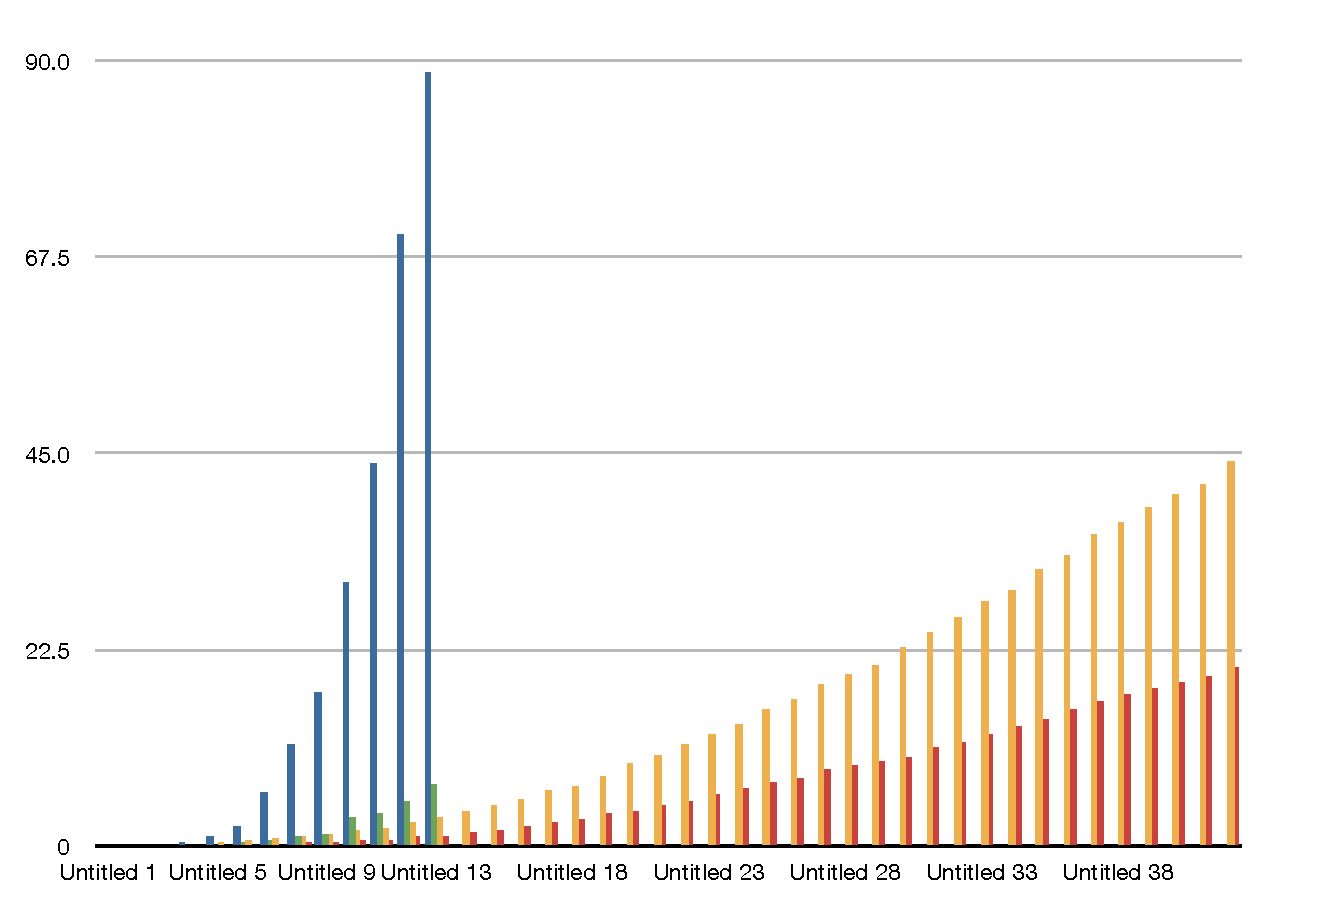
\includegraphics[width=1\columnwidth]{pic-runtime-buttons}
  \caption{Runtimes of FF and SGPLAN on the minimal GIVE worlds for $h=20$. The horizontal axis is $n$, ranging from 1 to 40.}
  \label{fig:give-runtime-minimal}
\end{figure}


\subsection{Experiment 3: GIVE worlds with extra positions}
\label{sec:experiment-3:-give}

In the final experiment, we vary the structure of the GIVE world in order
to judge the effect that universe size has on the planning problem in this
domain.  Starting with the ordinary GIVE world described in Experiment~2,
we add another $w$ by $h$ empty ``junk'' positions to the right of the
minimal world (see Figure~\ref{fig:give-junk}). These new positions are not
actually needed in any plan, but approximate the situation in the actual
GIVE domain, where most grid positions never need to be used. We leave the
initial state and goal untouched. As before, we generate a GIVE world
description and then convert it into a planning problem.

\begin{figure}
  \centering
  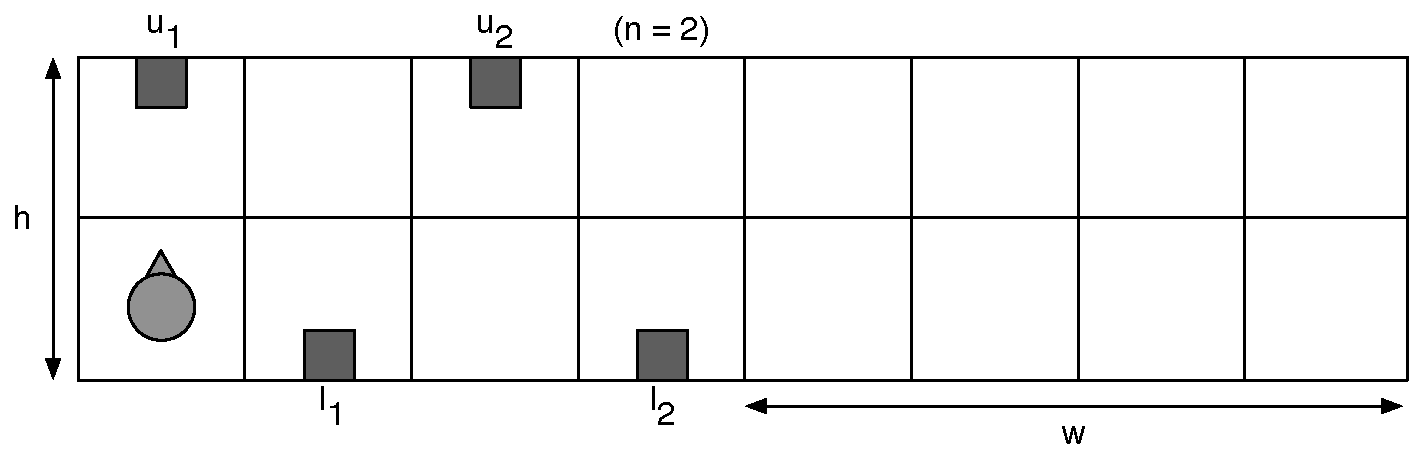
\includegraphics[width=1\columnwidth]{pic-empty-buttons}
  \caption{GIVE world with extra ``junk'' positions.}
  \label{fig:give-junk}
\end{figure}

Results for the $h=20$, $n=5$ case (with $w$ ranging from $1$ to $70$) are
shown in Figure~\ref{fig:give-runtime-junk}. As in Experiment~2, FF again
runs out of memory, this time at $w=17$. SGPLAN happily solves inputs
beyond $w=70$. However, unlike in Experiment 2, both planners now spend a
substantial propertion of their time on grounding. In SGPLAN, this
translates to a ``parsing time'' (which \todo{presumably} includes
grounding) which grows from 180 ms to 21.7 seconds as $w$ grows from $1$ to
$75$. The rest of the runtime (which also includes the search time) only
grows from 400 ms to 2.3 seconds. This difference is particularly dramatic
given that the actual optimal plan in each case is an identical plan of
about 100 steps. The planning times for these instances are also concerning
since times over a couple seconds negatively affect the overall response
time of the system, which must react in real time to user actions.

\begin{figure}
  \centering
  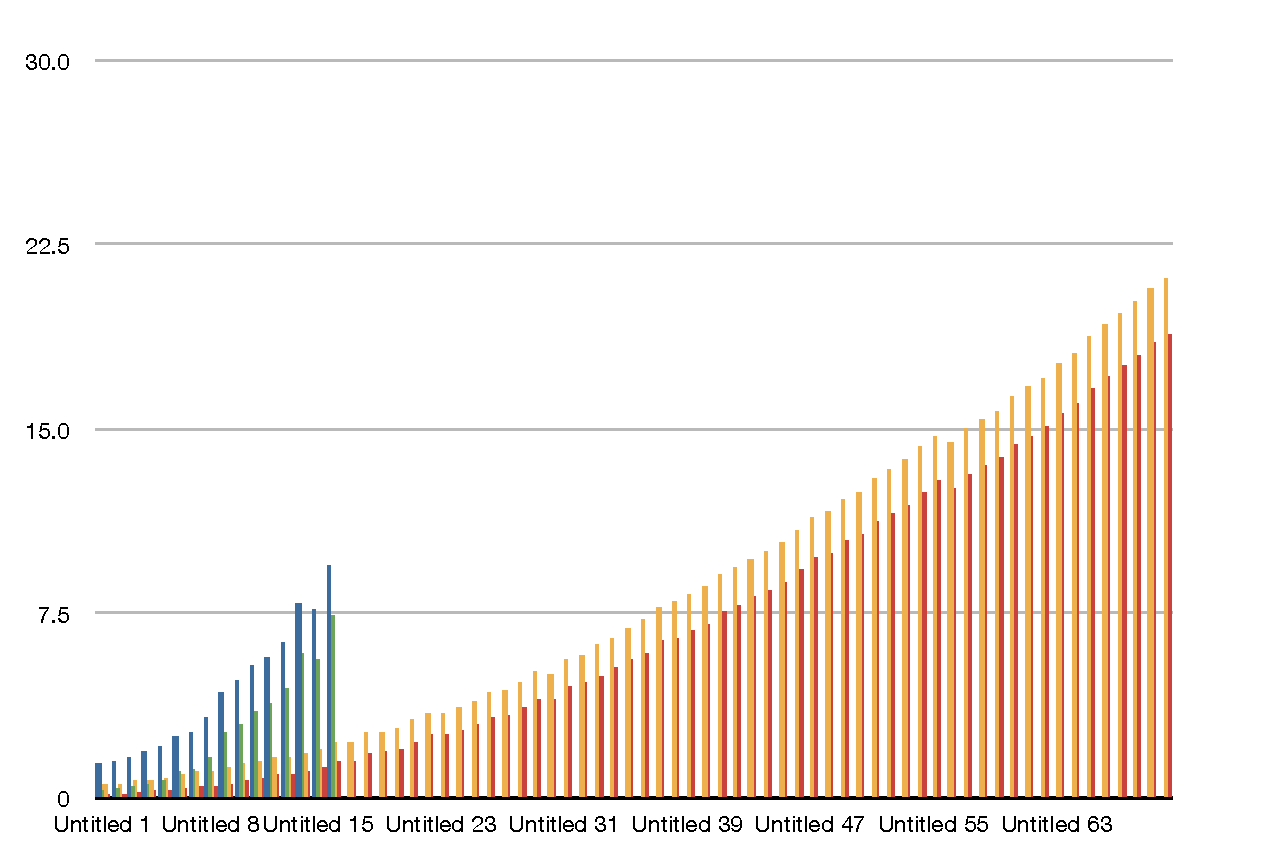
\includegraphics[width=1\columnwidth]{pic-runtime-empty-world}
  \caption{Runtimes of FF and SGPLAN on the GIVE worlds with junk
    positions for $h=20$ and $n=5$. The horizontal axis is $w$,
    ranging from 1 to 70.}
  \label{fig:give-runtime-junk}
\end{figure}


%%% Local Variables: 
%%% mode: latex
%%% TeX-master: "experiences"
%%% End: 
 % Experiments
\section{Conclusion} \label{sec:conclusion}


%%% Local Variables: 
%%% mode: latex
%%% TeX-master: "dl-gre-08"
%%% End: 


\bibliographystyle{naaclhlt2010}
\bibliography{literature}

\end{document}
